\section{Faktoren des Klimasystems}
% Abbildung, die nach und nach wächst, mit den erklärten Teilbereichen

% vgl IPCC AR5 climate feedbacks, AR4 chapter 1 basics: carbon cycle

\begin{frame}
  \frametitle{Faktoren des Klimasystems}
  \begin{columns}
  	\column{0.4\linewidth}
	Atmosphäre \\
	Hydrosphäre = Ozeane und Wasserkreislauf \\
	Kryosphäre = Eismassen \\
	Biospähre = Tiere und Pflanzen \\
	Pedosphäre = Boden \\
	Lithosphäre = Gestein 
	\column{0.6\linewidth}
	\begin{figure}
	 	\centering
	 	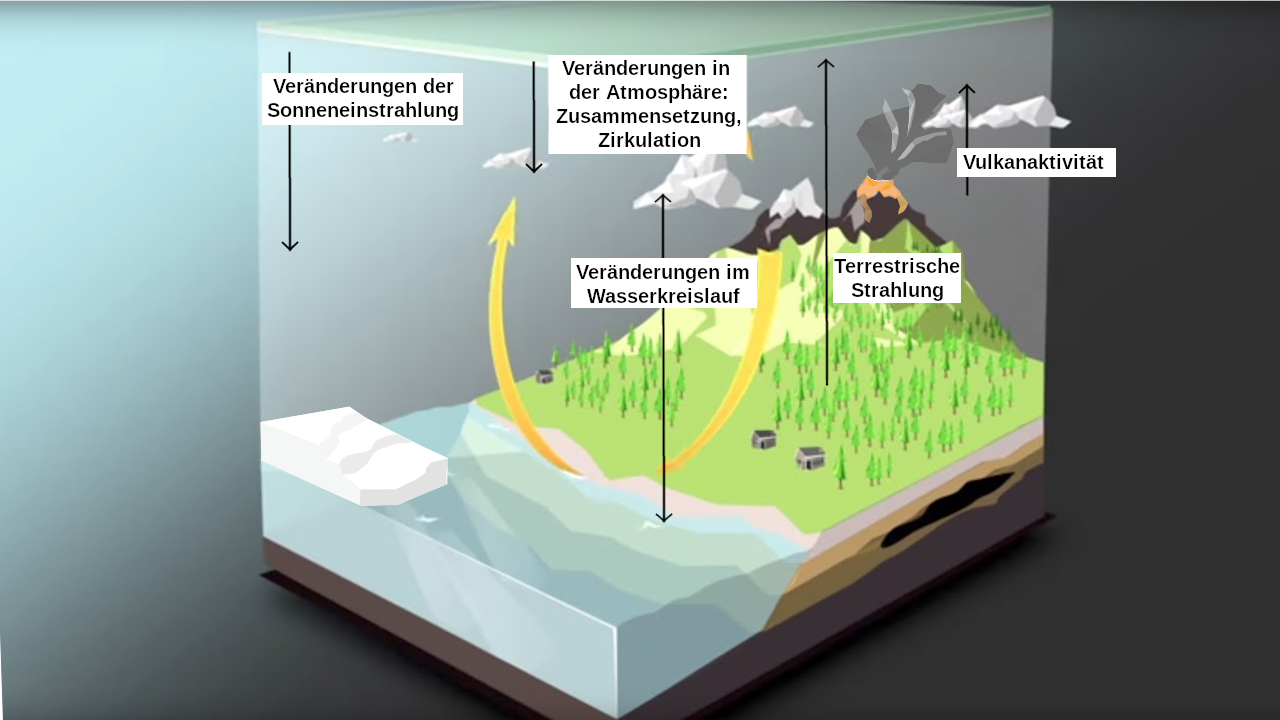
\includegraphics[width=0.8\linewidth]{bilder/WMO_Cycles_factors_general.png}
	 	\caption{Schematische Abbildung des Klimasystems, Quelle: IPCC 2007, Kapitel 1 und WMO-Video: The Carbon Cycle} % Anmerkungen hinzugefügt nach 
	\end{figure}
	%TODO: Evtl Bezeichnungen in Bild einfügen anstatt separat auflisten
	\end{columns}

	\note{
	\begin{itemize}
		\item[] Wir fokussieren uns hier auf die Faktoren Hydrosphäre, Krysphäre und Biosphäre bzw. vor allem die Vegetation.
		\item[] Die Effekte in diesen Komponenten sind bereits heute spürbar: Dürreperioden und Überflutungen, Rückgang der Eisschilde und Waldrodung.
		\item[] Die Zustände der Böden sind aber entscheidend für die Vegetation und Landwirtschaft.
		\item[] $\rightarrow$ Erosion von Böden durch Übernutzung und Dürren macht sie unfruchtbar (Nährstoffverlust und Austrocknung).
		\item[] $\rightarrow$ Gestein liefert Mineralien, was ebenfalls für die Vegetation und auch z.B. Schalenbildung bei Muscheln wichtig ist.
	\end{itemize}
	}
\end{frame}


\begin{frame}
	\frametitle{Hydrosphäre - Wassermassen}
	\begin{figure}
		\centering
		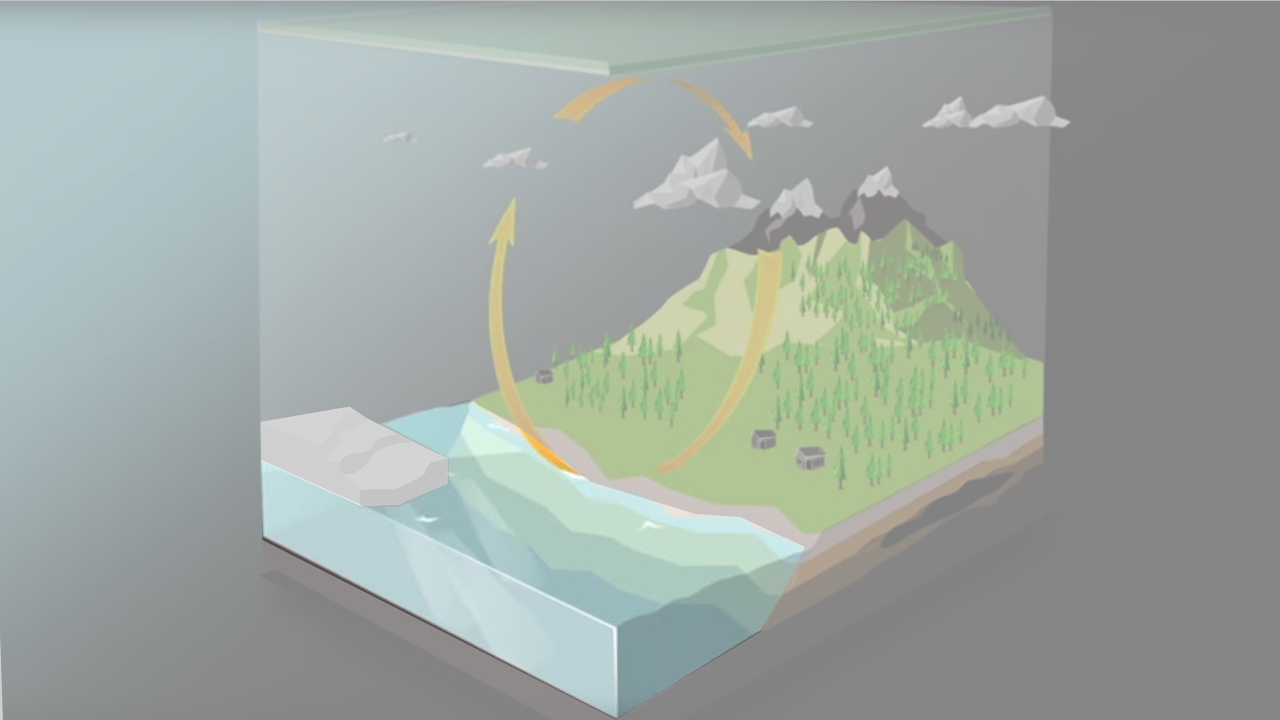
\includegraphics{bilder/WMO_Cycles_water.png}
		\caption{Etwa 2/3 der Erdoberfläche sind von Wasser bedeckt, somit ist die Hydrosphäre allein durch die Masse ein wichtiger Faktor des Klimasystems.}
	\end{figure}

	\note{
	\begin{itemize}
		\item[] Etwa 2/3 der Erdoberfläche sind von Wasser bedeckt, somit ist die Hydrosphäre allein durch die Masse ein wichtiger Faktor des Klimasystems.
		\item[] Daher widmen wir uns zuerst den Wassermassen.
	\end{itemize}
	}
\end{frame}


\begin{frame}
	\frametitle{Hydrosphäre - Wassermassen}
	\begin{itemize}
		% Aufteilung von https://www.lenntech.de/faq-wasser-menge.htm, aber auch Wetzel, Robert G. 1983 in "Periphyton of freshwater ecosystems"
		\item Ozeane - Salzwasser ca. 97\,\%
		\item Flüsse und Seen - Süßwasser $<$ 1\,\%
		\item Eismassen ca. 2\,\% % zu den Eismassen gibt es einen extra Abschnitt
	\end{itemize}

	\note{
		\begin{itemize}
			\item[] Der Großteil der Wassermassen ist Salzwasser.
			\item[] Süßwasser bildet nur weniger als 1\% des globalen Wassers.
			\item[] Eismassen machen 2\% des Wassers aus und binden den größten Teil des Süßwassers, da das Salz bei der Eisbildung abgespalten wird.
			\item[] Allerdings betrachten wir das Eis erst etwas später.
		\end{itemize}
	}
\end{frame}


\begin{frame}
	\frametitle{Strahlungseigenschaft des Wassers} % M.Latif Klimawandel und Klimadynamik S. 23
	\begin{itemize}
		\item Wasser ist ein Dipol-Molekül \textcolor{blue}{$H_2O$}
		\begin{itemize}			
			\item[$\rightarrow$] Kann wirksam Infrarotstrahlung absorbieren
			\item[$\rightarrow$] Kann viel Wärme aufnehmen bevor es verdampft $\rightarrow$ "Trägheit"
		\end{itemize}
		
		%Allgemein liegt die größte Dichte des Wassers bei 4 Grad
		\item<3-> Größte Dichte von reinem Wasser bei \SI{4}{\degreeCelsius}
		\begin{itemize}
			\item<2->[$\rightarrow$] Eis schwimmt auf Wasser
		\end{itemize}		
		% Im besonderen Fall des Salzwassers liegt die größte Dichte jedoch bei -3.8 Grad
		\item<5->Größte Dichte von Salzwasser bei \SI{-3,8}{\degreeCelsius}
		\begin{itemize}
			\item<3-> [] Bei der Eisbildung wird Salz freigesetzt
			\item<3-> [$\rightarrow$] Wasser kann kälter werden und sinkt in die tieferen Schichten des Ozeans
			\item<3-> [$\rightarrow$] Wärmeres, weniger dichtes Wasser steigt auf
			\item<3-> [] \textbf{\textcolor{blue}{Konvektion}} in den Polarregionen 
			\item<3-> [$\rightarrow$] Kohlenstoffsenken
		\end{itemize}
	\end{itemize}

% TODO: evtl. Abbildung der Konvektion: Abgabe von Wärme bei Aufnahme von atmosphärischen Gasen, die dann in die Tiefsee gelangen und dort gespeichert werden

%TODO: Erklärung von Senken
\end{frame}

\begin{frame}
	\frametitle{Wasserdynamik} %M. Latif Klimawandel und Klimadynamik S.24
	\begin{block}{Windgetriebene Zirkulation: } % eher horizontal
		Oberflächenströmung der Ozeane durch Reibung, Erdrotation (Corioliskraft) und Form der Meeresbecken 
	\end{block}
	\begin{block}{Dichtegetriebene Zirkulation: }  % eher vertikal
		Erwärmung, Abkühlung, und Änderung des Salzgehaltes (durch Eisbildung, Verdunstung oder Niederschlag) haben Einfluss auf die Dichte des Wassers, wodurch die Wassermassen zirkulieren
	\end{block}

	\note{
		\begin{itemize}
			\item[] Die großen Wassermassen der Ozeane haben eine bestimmte Strömung, z.B. Golfstrom von der Arktis über die Küste Mexikos bis an die Antarktis.
			\item[] Die Stömung ergibt sich vorallem durch die Erdrotation (Corioliskraft).
			\item[] Die oberflächliche Strömung der oberen 100 Meter entsteht durch Wind (und darauf resultierende Reibung) und die Form der Meeresbecken.
			\item[] Die Tiefenströmung wird durch die Konvektion angetrieben. Die Dichte des Wassers spielt dabei eine entschiedende Rolle, da dichteres Wasser nach unten sinkt und leichteres empor steigt.
			\item[] Warme Temperaturen führen zum aufwärem des Oberflächenwassers und damit zu einer geringeren Dichte.
			\item[] Dadurch werden Oberflächenwasser und Tiefenwasser stark getrennt - und somit strömen die Wassermassen mit unterschiedlicher Geschwindigkeit.
		\end{itemize}
	}

\end{frame}


\begin{frame}
	\frametitle{Wirkung des Wassers auf das Klima}
	\begin{itemize}
	\item Ca. 70\,\% der Erdoberfläche ist mit Wasser bedeckt
	\item [$\rightarrow$] Die \textit{Trägheit} des Wassers ist ein entscheidender Faktor für die Trägheit des Klimas und der Klimaänderungen % M.Latif Klimawandel und Klimadynamik S. 23
	\item Kohlenstoffsenken in der Tiefsee können durch erwärmen der Ozeane \textit{irgendwann} freigesetzt werden
	\item[$\rightarrow$] massiver Anstieg des atmosphärischen $CO_2 \rightarrow$ Verstärkung des Treibhauseffekts
	\item Positive Verstärkung von $CO_2$ und Wasserdampf: eine wärmere Atmosphäre kann mehr Wasserdampf (und $CO_2$) aufnehmen
	\end{itemize}
\end{frame}

\begin{frame}
	\frametitle{Trägheit des Klimas}
	Die Trägheit des Klimas zeichnet sich dadurch aus, dass Feedbacks verzögert zu einem klimawirksamen Ereignis auftreten. Das heißt, die einzelnen Komponenten des Klimasystems benötigen eine gewisse Zeit sich in den veränderten Bedingungen des Systems zu stabilisieren
	
	\begin{figure}
		\centering
		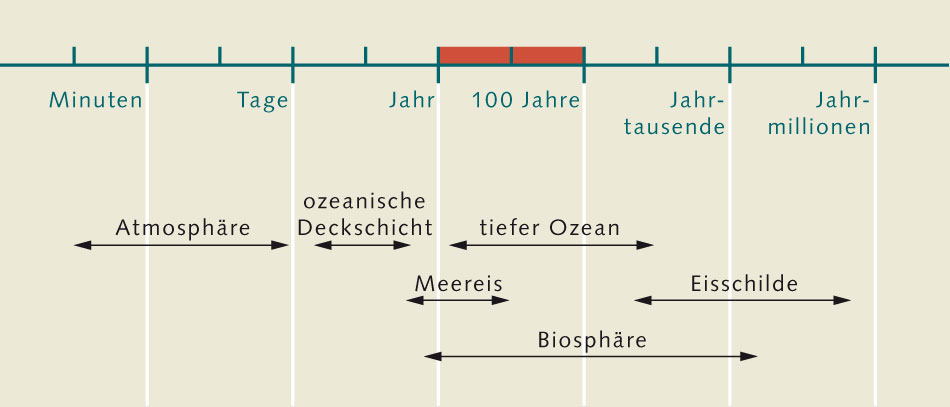
\includegraphics[width=0.8\linewidth]{bilder/zeitskala-klimasystem_world_ocean_review.jpg}
		\caption{Zeitskalen im Klimasystem, Quelle: maribus nach Meinecke und Latif, 1995}
		\label{fig:traegheit}
	\end{figure}
	
	Besonders die Ozeane und Eisschilde benötigen demnach eine sehr lange Zeit, um sich geänderten klimatischen Bedingungen anzupassen.
	
	\note{
		\begin{itemize}
			\item[] Gerade habe ich ja schon gesagt, dass die Trägheit des Wassers entschiedent ist. Das zeigt sich nun auch in dieser Abbildung.
			\item[] Die Wassermassen sind in dieser Abbildung stark vertreten.
			
			\item[] Die untere Atmosphäre passt sich innerhalb weniger Stunden den Bedingungen der Erdoberfläche an (Temeperatur, Gase, etc.)
			\item[] Die Wassermassen reagieren sehr unterschiedlich auf geänderte Umgebungsbedingungen.
			\item[] Flüsse, Seen und Oberflächenwasser wärmen sich dabei deutlich schneller auf als die tierefen Ozeanschichten. (Das kennt man vielleicht aus Badeseen - die oberen 50 cm sind angenehm warm und darunter liegt deutlich kälteres Wasser)
			\item[] Besonders unterschiedlich schnell reagiert die Biosphäre. Graslandschaften können schnell austrocken, Wälder dagegen verändern sich über Jahrtausende hinweg. Die Vegetation bestimmt in vielen Fällen auch die Ansiedlung von Lebewesen. Die Änderung der Vegetation kann das Ende des Lebenraums einiger Lebewesen bedeuten, aber auch neue Ansiedluneg bedingen.
			\item[] Eine besonders lange Reaktionszeit haben die Eisschilde der Erde. Auf die Eismassen gehen wir als nächstes ein.
		\end{itemize}
	}
\end{frame}

\begin{frame}
	\frametitle{Kryosphäre - Eismassen}
	
	\begin{figure}
		\centering
		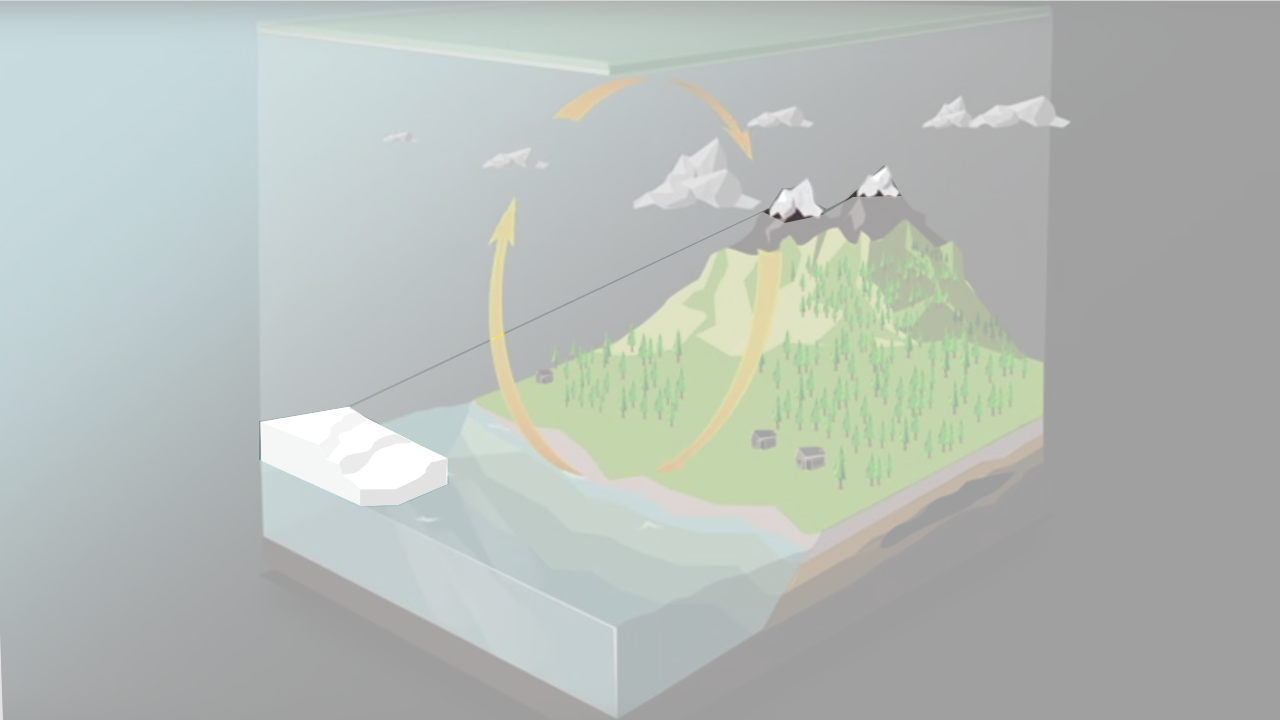
\includegraphics{bilder/WMO_Cycles_ice.png}
		\caption{Kryosphäre umfasst alle Formen und Schnee und Eis}
	\end{figure}
\end{frame}

\begin{frame}
	\frametitle{Kryosphäre - Eismassen} % Eismassen der Erde
	\begin{itemize}
		\item ca. 2\,\% des Wassers ist in fester Form in Gletschern und an den Polkappen dauerhaft gebunden.
%		\item  inländische Eisflächen speichern ca. 75\% des globalen Süßwassers
		\item Eis reflektiert die ankommende Sonnenstrahlung zu großen Teilen
		$\rightarrow$ \textbf{\textcolor{blue}{Albedo-Effekt}}\\
		
		\item Je weniger Eismassen, desto weniger Strahlung wird reflektiert und bleibt in der Atmosphäre $\rightarrow$ Verstärkung des Treibhauseffekts
		
		\item Durch Rußablagerungen auf den Eismassen wird mehr Sonnenstrahlung absorbiert ("Black Carbon")
		 $\rightarrow$ Schmelzen des Eis und Verringerung des Albedo-Effekts % (Nature Geoscience, 2014; doi: 10.1038/ngeo2180) 
	\end{itemize}
	
\end{frame}

\begin{frame}
	\frametitle{Kryosphäre - Komponenten}
	Die größten Komponenten der Kryosphäre sind: 
	\begin{itemize}
		\item Meereis: schwimmende Eismassen, 19-27 km$^2$
		\item Eisschilde: über Grönland und der Antarktis, 14 km$^2$
		\item Permafrost: gefrorene Böden, 22,8 km$^2$
	\end{itemize}
	
	\glqq Ein einmal eingesetzter Rückzug großer kontinentaler Eisschilde kann selbst nach Stabilisierung der Randbedingungen [($CO_2$-Emissionen)] über ein Jahrtausend lang anhalten\grqq{} (Latif, 2009 und IPCC, 2001)\\
	$\rightarrow$ siehe auch: Trägheit des Klimas in Abbildung \ref{fig:traegheit}
\end{frame}

\begin{frame}
	\frametitle{Meereis}
	\begin{itemize}
		\item bildet die Grenze zwischen Ozeanen und Atmosphäre
		\item Luft über dem Meereis ist deutlich kälter als über dem offenen Ozean 
		\item [$\rightarrow$] Abkühlung der Polarregionen und Verstärkung der atmosphärischen Zirkulation (Winde)
		\item [$\rightarrow$] beeinflusst Konvektion: je weniger Eis, desto schwächer die Konvektion, desto schwächer sind (langfristig) ozeanische Strömungen 
	\end{itemize}
\end{frame}

\begin{frame}
	\frametitle{Eisschilde}
	\begin{itemize}
		\item Volumen: 25 km$^3$ (Antarktis) + 3 km$^3$ (Grönland) = 28 km$^3$
		\item ihre Masse wird durch Niederschlag, Lufttemperatur und Strahlung bestimmt % (je mehr Schnee, desto mehr Eis kann sich bilden)
		\item in der Antarktis gibt es Ausläufer des Landeises auf den Ozean hinaus (Schelfeis) $\rightarrow$ 0,7 km$^3$
%		\item tiefer liegende Schichten der Eisschilde schmelzen durch den Druck auf die Landmassen $\rightarrow$ erzeugt Spannungen im Eis
		\item Eisschilde schmelzen an randnahen Bereichen
		\item durch die höheren Temperaturen im Sommer auf der Nordhalbkugel ist das grönländische Eisschild besonders von einer Erwärmung gefährdet
		\item \textbf{Eisschilde haben das größte Potential für einen Anstieg des Meeresspiegels, da sie nicht - wie das Meereis - zum Meeresspiegel beitragen}
	\end{itemize}
\end{frame}

\begin{frame}
	\frametitle{Permafrost}
	\begin{itemize}
		\item dauerhaft gefrorene Böden durch dauerhaft kalte ($<$ \SI{0}{\degreeCelsius}) Temperaturen
		\item größtenteils in Nordamerika und Eurasien
		\item zum Teil mehrere hundert Meter tief gefroren %(z.B. in Sibirien, da dort kaum Schnee die Böden vor der Kälte schützt)
		\item Konservierung unzersetzter organischer Materie
		\item [$\rightarrow$] geschätzte Menge an gespeichertem Kohlenstoff: 1000 Gt (1 Gt = $10^15$ g)
		\item deutliche Verschiebung der Permafrostgrenze im letzten Jahrhundert beobachtet %(z.B. in Kanada um ca. 100 km nach Norden)
		\item die globale Erwärmung gefährdet den Fortbestand von Permafrost 
		\item Folgen des Abtauen: Absenken der Böden, Überschwemmungen, Zersetzung bisher konservierter Materie $\rightarrow$ Freisetzung großen Mengen $CO_2$ und Methan
		\item Wissenschaft nimmt an, dass deutlich mehr Treibhausgase freigesetzt werden als die erwartete neue Vegetation binden würde
	\end{itemize}
\end{frame}

\begin{frame}
	\frametitle{Konsequenzen der Verringerung der Eismassen}
	\begin{itemize}
		\item verringerter Albedo-Effekt
		\item abgeschwächte Konvektion
		\item abgeschwächte Ozeanströmung und Winde
		\item massive Freisetzung von Treibhausgasen aus den Senken Ozean und Permafrost
		\item Trägheit führt zu verzögertem Eintreten der Änderungen
	\end{itemize}
	
	$\rightarrow$ insgesamt: eine Verstärkung des Treibhauseffekt mit weiteren noch unabsehbaren Folgen
\end{frame}

\begin{frame}
	\frametitle{Interaktion Hydrosphäre, Kryosphäre und Atmosphäre}
	\begin{figure}
		\centering
		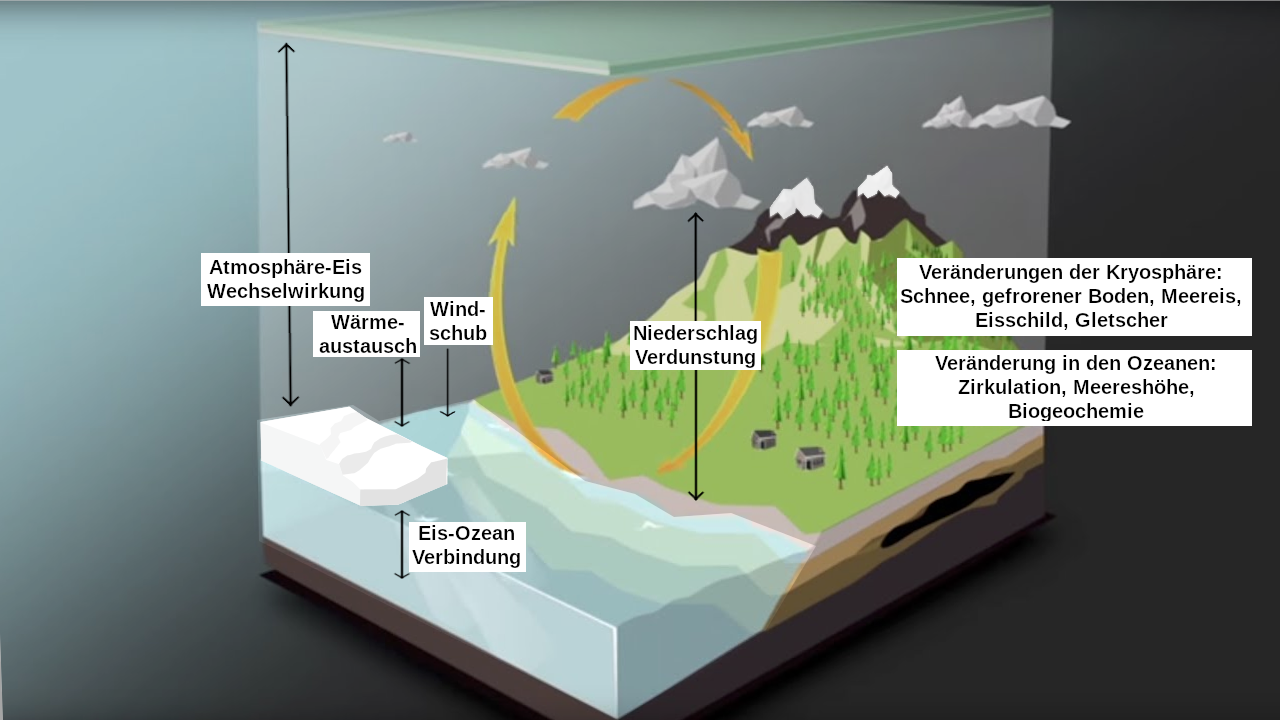
\includegraphics{bilder/WMO_Cycles_factors_waterAndIce.png}
		\caption{Interaktion Hydrosphäre, Kryosphäre und Atmosphäre}
	\end{figure}
\end{frame}

\begin{frame}
	\frametitle{Vegetation}
	
	\begin{figure}
		\centering
		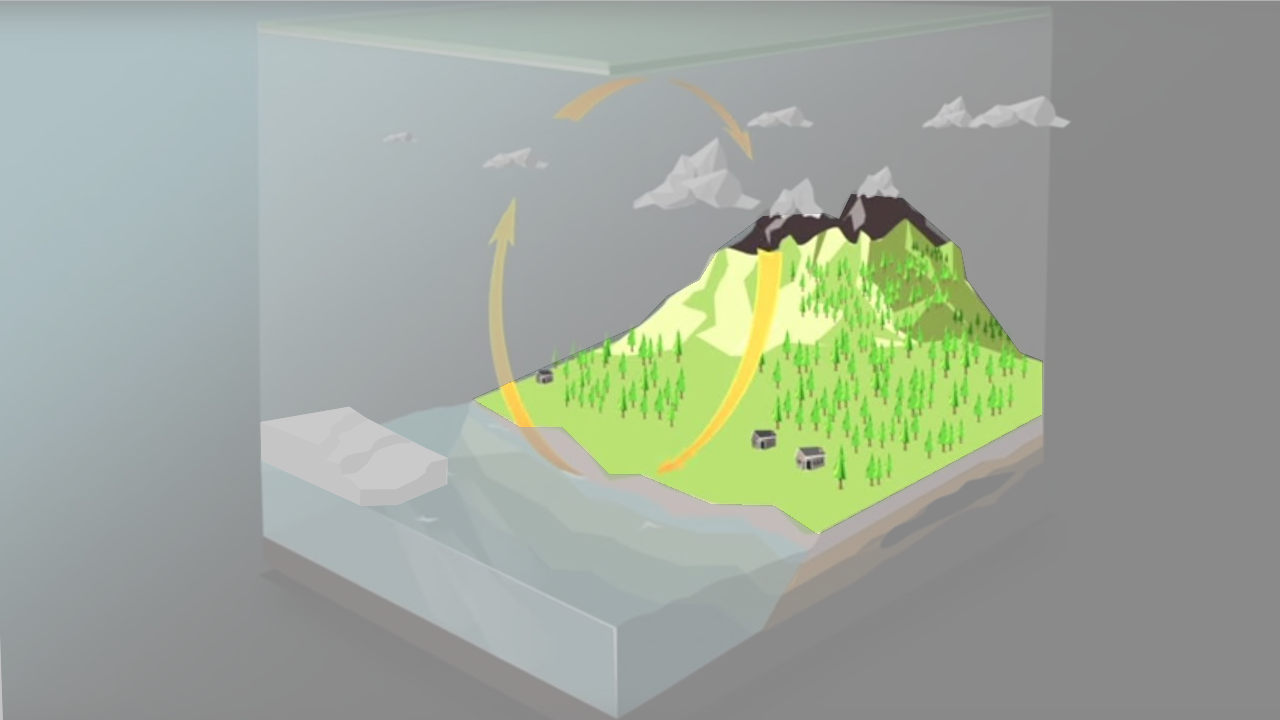
\includegraphics{bilder/WMO_Cycles_land.png}
		\caption{Die Vegetation ist eine interaktive Komponente des Klimasystems}
	\end{figure}
\end{frame}

\begin{frame}
	\frametitle{Vegetation}
		%TODO -z.B. in  M.Latif: Kap 1.3.4
		\begin{itemize}
%			\item beeinflusst u.a. Wasserkreislauf, Strahlungshaushalt und Stoffkreisläufe:
			\item Bodenbedeckung wirkt auf Wind, Wasseraustausch und Strahlungshaushalt
			\item [$\rightarrow$] Wälder bremsen Winde, speichern Wasser, beeinflussen Wolkenbildung und bilden Schatten und großen Lebensraum
			\item [$\rightarrow$] in Wüsten und Steppen versickert Wasser schneller und es gibt kaum Schatten, dafür existiert schwacher Albedo-Effekt
			\item Existenz und Wachstum von Vegetation bindet u.a. $CO_2$ und absorbiert Strahlung
			\item Absterben von Vegetation führt zu Freisetzung von $CO_2$ und anderen Stoffen in die Luft und Böden % Nitrat, Phosphat, Stickstoff etc.
		\end{itemize}
\end{frame}


\begin{frame}
	\frametitle{Interaktion Vegetation und Atmosphäre}
	
		\begin{figure}
		\centering
		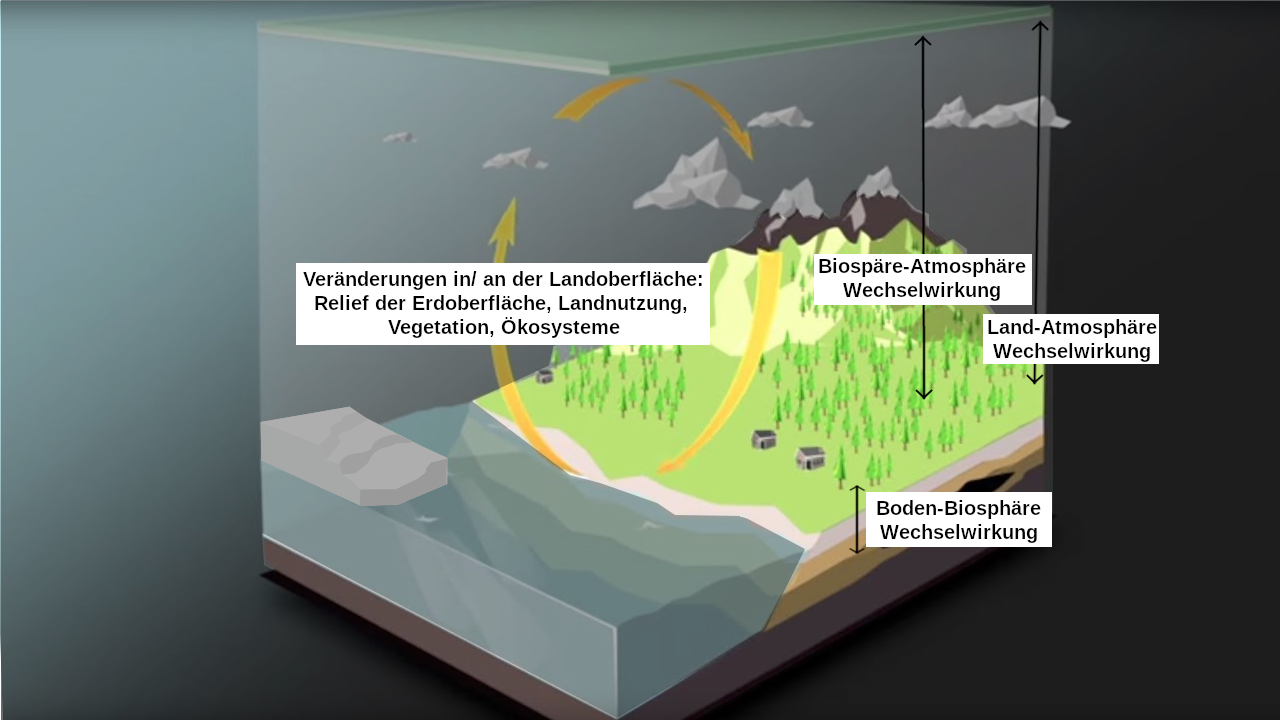
\includegraphics{bilder/WMO_Cycles_factors_landAndGround.png}
		\caption{Interaktion der Biosphäre und Atmosphäre}
	\end{figure}

\end{frame}



\begin{frame}
	\frametitle{Das Klimasystem - Zusammenfassung}
	% Abbildung mit allen zuvor erklärten Elementen
	
	\begin{figure}
		\centering
		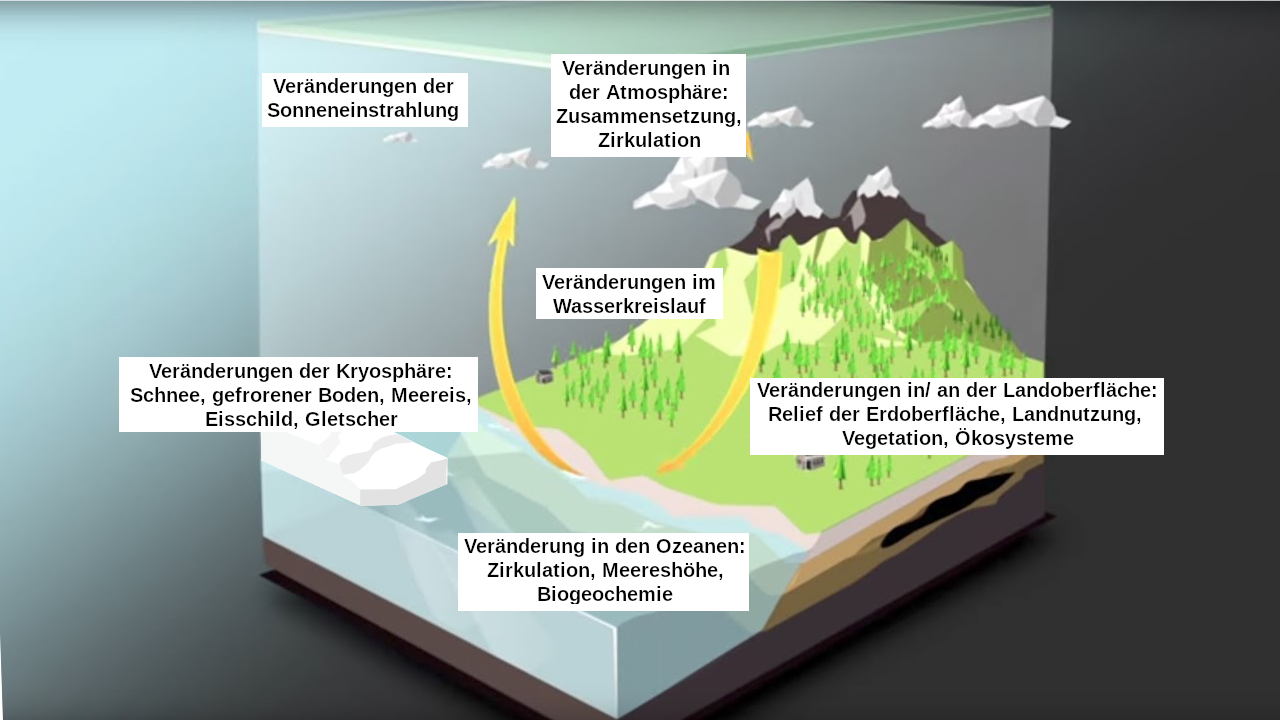
\includegraphics{bilder/WMO_Cycles_overview.png}
		\caption{Abbildung des Klimasystems mit allen zuvor erklärten Elementen}
	\end{figure}
\end{frame}


\begin{frame}
	\frametitle{Kohlenstoffkreislauf}
	
	% nach der Vegetation und Lebewesen
	% --> mit Fokus Fabriken und Ausstoß von CO2
	\begin{columns}
		\column{0.6\linewidth}		
		\begin{figure}
			\centering
			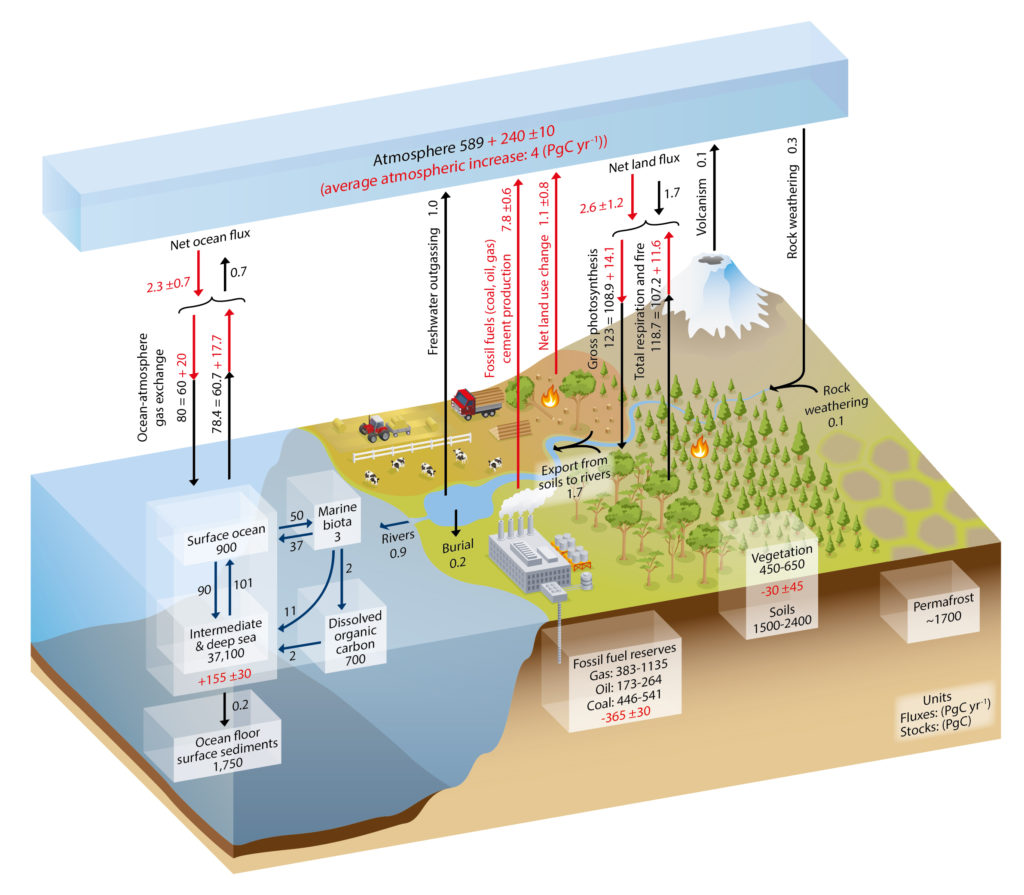
\includegraphics[width=0.9\linewidth]{bilder/IPCC_Cycles_carbon.jpg}
			\caption{Vereinfachte Abbildung zum jährlichen Kohlenstoffkreislauf, Quelle: IPCC 2014, Kapitel 6}
		\end{figure}
		\column{0.4\linewidth}
		$\Rightarrow$ vermutete natürliche $CO_2$-Flüsse vor der Industrialisierung (vor 1750)\\
		\color{red}$\Rightarrow${ }\color{black} durch Menschen verursachte mittlere jährliche $CO_2$-Flüsse (2000 - 2009) \\% es ist anzunehmen, dass die Werte heute nochmal höher sind als die angegebenen
		\color{red}\textbf{rote Reservoire}\color{black}: kumulative Änderung zwischen 1750 und 2011
		\begin{center}
			$\downarrow$
		\end{center}
		\textbf{der Kohlenstoffgehalt der Atmosphäre steigt um ca. 4 Gt pro Jahr}
	\end{columns}
	% Wichtig hierbei ist vorallem das Fazit, dass der CO2 Gehalt der Atmosphäre sich seit der Industrialisierung beinahe verdoppelt hat!
\end{frame}

\begin{frame}
	\frametitle{Kohlenstoffkreislauf - Der Faktor Mensch}
	\begin{itemize}
		\item $CO_2$ ist das wichtigste Spurengas des menschengemachten Treibhauseffekts
		\item es gelangt durch Verbrennung fossiler Brennstoffe vermehrt in die Atmosphäre
		\item ca. 80\% der gestiegenen $CO_2$ Konzentration der Atmosphäre lassen sich auf Verbrennung zurückführen
		\item der restliche Anteil fällt auf die Änderung der Landnutzung, v.a. die Brandrodung
		\item Rückführung auf den Menschen durch Messung von Kohlenstoffisotopen (Anzahl Neutronen in einem Kohlenstoffatom)
		% C12 hat sechs und C13 sieben Neutronen, beide haben 6 Protonen, die den Kohlenstoff kennzeichnen
		\item [$\rightarrow$] das Verhältnis der Isotope in fossilen Brennstoffen hat durch die Verbrennung Einfluss auf das Verhältnis in der Atmosphäre
	\end{itemize}
\end{frame}


% Aber nicht nur der CO2 Gehalt der Atmosphäre hat sich erhöht, sondern auch der von Methan und Lachgas:
\begin{frame}
	\frametitle{Atmosphärisches Methan und Lachgas}
	
	% nach der Vegetation und Lebewesen
	% --> mit Fokus Fabriken und Ausstoß von CO2
	
	\begin{figure}
		\begin{columns}
			\column{0.5\linewidth}
				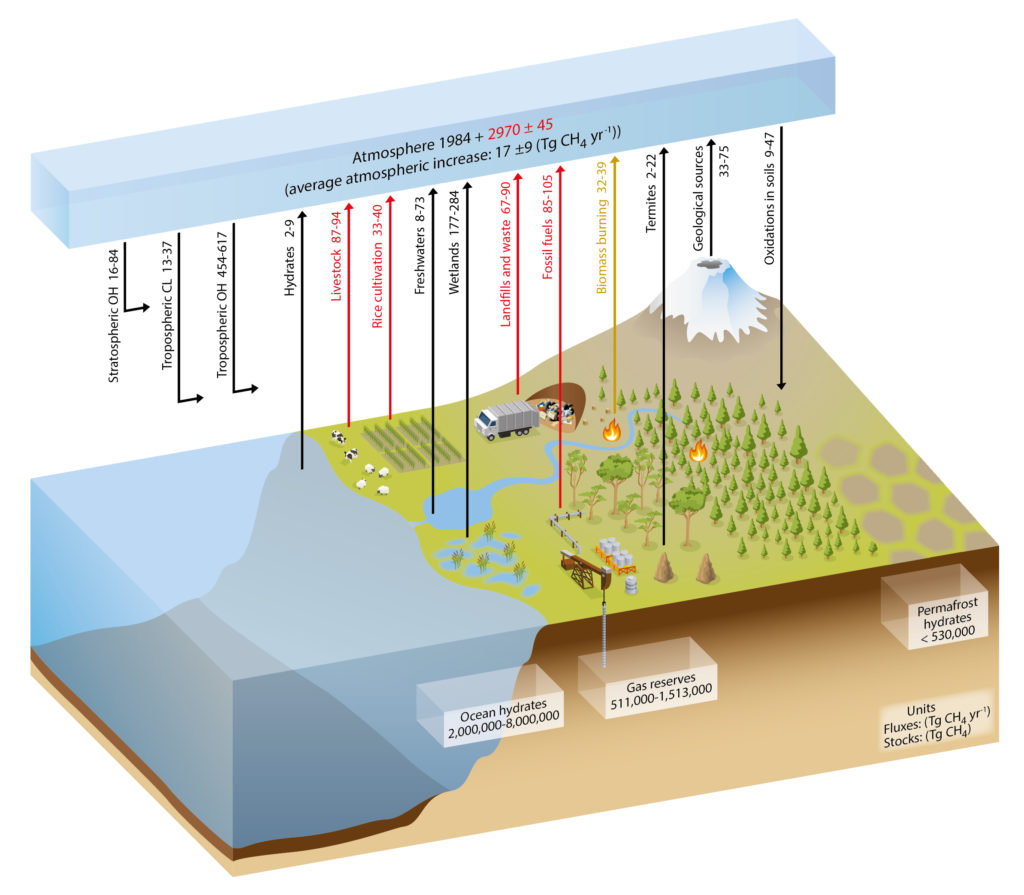
\includegraphics[width=\linewidth]{bilder/IPCC_Cycles_methane.jpg}
			
			\column{0.5\linewidth}
				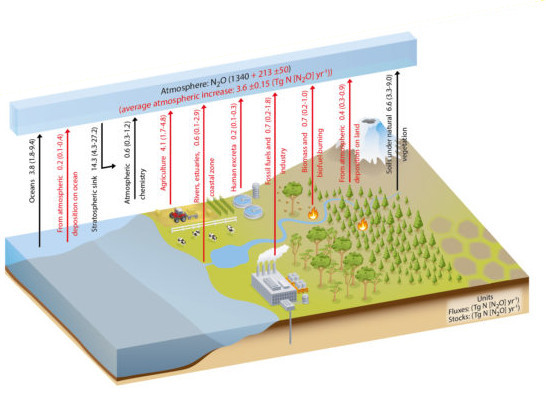
\includegraphics[width=1.1\linewidth]{bilder/IPCC_Cycles_n2o_.jpg}
		\end{columns}
		\caption{Vereinfachte Abbildung zum Methan- und Lachgaskreislauf, Quelle: IPCC 2014, Kapitel 6}
	\end{figure}

	\vspace{-1cm}
	Der Gehalt an Methan in der Atmosphäre hat sich zwischen 1750 und 2011 um 250 \,\% erhöht, der Gehalt von Lachgas um etwa 20 \,\%

\end{frame}

\begin{frame}
	\frametitle{Zusammenfassung}
	\begin{itemize}
		\item Klima ist der mittlere Zustand der Atmosphäre an einem bestimmten Ort über einen längeren Zeitraum
		\item Atmosphäre und Strahlungshaushalt der Erde erzeugen lebensfreundliche Bedingungen auf der Erde
		\item Der natürliche Treibhauseffekt entsteht vorallem durch Wasserdampf und $CO_2$.
		\item $CO_2$, $CH_4$ und $N_2O$ sind starke Treibhausgase
		\item Durch den Anstieg der atmosphärischen Konzentrationen dieser drei seit der Industrialisierung kann der Mensch als Ursache angenommen werden.
		\item Die Komponenten des Klimasystems hängen stark zusammen, sodass Veränderungen eines Faktors zum Teil deutliche Folgen in anderen Bereichen erzeugen kann.
		\item Manche Änderungen treten erst nach hunderten Jahren auf, manche sind aber auch schon heute und in wenigen Jahren spürbar!
	\end{itemize}
\end{frame}

\begin{frame}
	\frametitle{Zusammenfassung und Ausblick}
	\begin{figure}
		\centering
		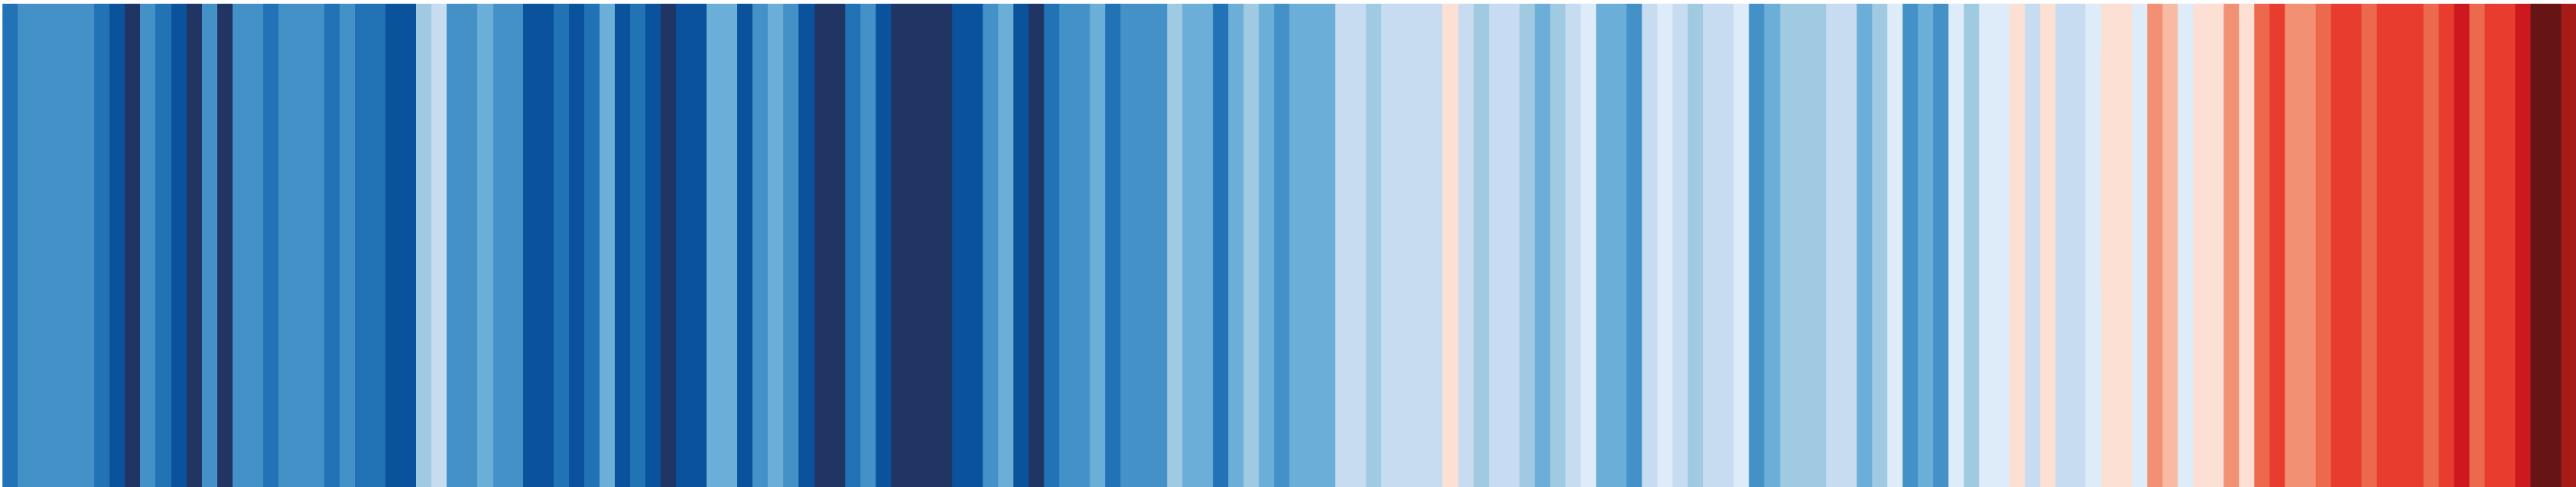
\includegraphics[width=\linewidth]{bilder/s4f-warming-stripes}
		\caption{Die Warming Stripes}
	\end{figure}
	$\rightarrow$ Die langfristige Erwärmung und Häufung extremer Wetterereignisse bedeutet eine Veränderung des Klimas!\\
	$\rightarrow$ Viele dieser Änderungen sind in Modellen der Klimaforscher relativ genau vorherzusagen. \\
	$\rightarrow$ Das Ausmaß einiger Änderungen sind aufgrund der langfristigen Effekte nicht konkret vorherzusagen, aber die Tendenz ist klar.
\end{frame}

\begin{frame}
	\frametitle{Referenzen}
	\small{
	\textbf{Bildungsserver Hamburg,} Hamburger Bildungsserver (HBS), https://bildungsserver.hamburg.de/klimawandel/ \\
	
	\textbf{IPCC, 2001:} Climate Change 2001: The Scientific Basis. Contribution of Working Group I to the Third Assessment Report of theIntergovernmental Panel on Climate Change[Houghton, J.T., Y. Ding, D.J. Griggs, M. Noguer, P.J. van der Linden, X. Dai, K.Maskell, and C.A. Johnson (eds.)]. Cambridge University Press, Cambridge, United Kingdom and New York, NY, USA, 881pp., https://www.ipcc.ch/report/ar3/wg1/\\
	
	\textbf{IPCC 2007:} IPCC, 2007: Climate Change 2007: The Physical Science Basis. Contribution of Working Group I to the Fourth Assessment Report of the Intergovernmental Panel on Climate Change [Solomon, S., D. Qin, M. Manning, Z. Chen, M. Marquis, K.B. Averyt, M. Tignor and H.L. Miller (eds.)]. Cambridge University Press, Cambridge, United Kingdom and New York, NY, USA, 996 pp.,  https://www.ipcc.ch/report/ar4/wg1/\\
	
	\textbf{IPCC, 2014:} IPCC, 2013: Climate Change 2013: The Physical Science Basis. Contribution of Working Group I to the Fifth Assessment Report of the Intergovernmental Panel on Climate Change [Stocker, T.F., D. Qin, G.-K. Plattner, M. Tignor, S.K. Allen, J. Boschung, A. Nauels, Y. Xia, V. Bex and P.M. Midgley (eds.)]. Cambridge University Press, Cambridge, United Kingdom and New York, NY, USA, 1535 pp., https://www.ipcc.ch/report/ar5/wg1/\\
	
	}
\end{frame}

\begin{frame}
	\frametitle{Referenzen}
	\small{
	\textbf{Mojib Latif}, Klimawandel und Klimadynamik, 2009, UTB GmbH, Auflage: 1, ISBN 978-3-8252-3178-1\\
	\textbf{S4F}, Scientists for Future, https://www.scientists4future.org/\\
	\textbf{WMO}, World Meteorological Organization, Video zum Kohlenstoffkreislauf: https://www.youtube.com/watch?v=E8Y6L5TI\_94
	}
\end{frame}